%!TEX root=../document.tex

\section{Ergebnisse}
\label{sec:Ergebnisse}

\subsection{Datenbank}
Es handelt sich hierbei um  Datenbank welche alle möglichen Daten in einem DVD-Store speichert. Es ist eine sehr große Datenbank, mit sehr vielen Daten, wobei sensitive Daten (Name, Email, Telefonnummer) mit einem Hash zensiert wurden.
\subsubsection{Einspielen}
Der erste Schritt war es einer Docker-Instanz anzulegen, auf welcher die Datenbank dann eingespielt wird. Es wurde eine simple postgres-Docker Instanz erstellt mit:

\begin{lstlisting}[language=bash]
docker run --name psql -v pgdata -d postgres
\end{lstlisting}

Wobei mit \verb|-v| eine docker Volume ausgewählt wird, welche mit: 

\begin{lstlisting}[language=bash]
docker volume create pgdata
\end{lstlisting}

erstellt wurde. Dies garantiert eine persistente Datenbank um Änderungen gespeichert zu halten. 

Nun wurde ein Nutzer namens \textbf{ds2} mit dem Passwort \textbf{ds2} angelegt, damit sich das Script, welches später ausgeführt wird, an die Datenbank anbinden kann und den \textbf{ds2}  User verwendet um die Datenbank einzuladen.

Anschließend wurde folgendes Script ausgeführt, in welchem bereits die Anbindung für die Docker-Instanz angegeben wurde:

\begin{lstlisting}[language=bash]
REM pgsqlds2_create_all.sh
REM start in ./ds2/pgsqlds2
SET CONNSTR=-h localhost -p 5432
REM If using vFabrid Data Director vPostgres then connection string will look like this
REM CONNSTR="-h {cc25670-1854-4476-9764-c384759f93d}.10.10.10.10 -p 5432"
SET DBNAME=ds2
SET SYSDBA=ds2
SET PGPASSWORD=ds2
SET createlang plpgsql ds2
cd build
REM Assumes DB and SYSDBA are already created
REM If building on vFabric Data Director vPostgres then you will need to comment out
REM     pgsqlds2_create_db.sql line becuase the DB is already created
psql %CONNSTR% -U %SYSDBA% -d postgres < pgsqlds2_create_db.sql
psql %CONNSTR% -U %SYSDBA% -d %DBNAME% < pgsqlds2_delete_all.sql
psql %CONNSTR% -U %SYSDBA% -d %DBNAME% < pgsqlds2_create_tbl.sql
psql %CONNSTR% -U %SYSDBA% -d %DBNAME% < pgsqlds2_create_sp.sql
cd ../load/cust
psql %CONNSTR% -U %SYSDBA% -d %DBNAME% < pgsqlds2_load_cust.sql
cd ../orders
psql %CONNSTR% -U %SYSDBA% -d %DBNAME% < pgsqlds2_load_orders.sql 
psql %CONNSTR% -U %SYSDBA% -d %DBNAME% < pgsqlds2_load_orderlines.sql 
psql %CONNSTR% -U %SYSDBA% -d %DBNAME% < pgsqlds2_load_cust_hist.sql 
cd ../prod
psql %CONNSTR% -U %SYSDBA% -d %DBNAME% < pgsqlds2_load_prod.sql 
psql %CONNSTR% -U %SYSDBA% -d %DBNAME% < pgsqlds2_load_inv.sql 
cd ../../build
psql %CONNSTR% -U %SYSDBA% -d %DBNAME% < pgsqlds2_create_ind.sql
psql %CONNSTR% -U %SYSDBA% -d %DBNAME% < pgsqlds2_create_trig.sql
psql %CONNSTR% -U %SYSDBA% -d %DBNAME% < pgsqlds2_reset_seq.sql
psql %CONNSTR% -U %SYSDBA% -d %DBNAME% < pgsqlds2_create_user.sql
psql %CONNSTR% -U %SYSDBA% -d %DBNAME% -c "ANALYZE;"
\end{lstlisting} 

Nun konnte mit dem Befehl \verb|docker exec -ti psql bash| auf den Container zugegriffen werden. In diesem musste mit \verb|su postgres| auf den \textbf{postgres} Benutzer gewechselt, da auf die postgresql Datenbank innerhalb vom Container nicht mit \textbf{root} zugegriffen werden kann. 

Anschließend wurde mit dem Befehl \verb|psql| postgresql gestartet, mit \verb|\c ds2| in die Datenbank gewechselt und mit \verb|\dt| kann überprüft werden, ob die Einspielung funktioniert hat:

\begin{minipage}{\linewidth}
	\centering
	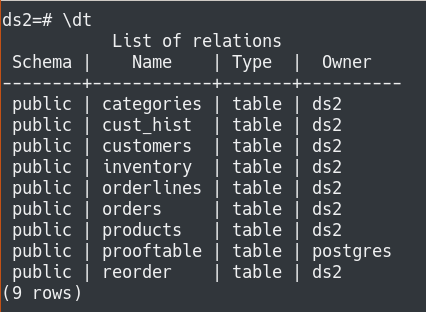
\includegraphics[width=0.8\linewidth]{images/table1}
	\figcaption{Datenbank wurde in das System eingespielt}
\end{minipage}
\subsubsection{Analysieren}
Um die Datenbank zu analysieren wurde \textbf{pgAdmin} lokal installiert, die Informationen der Datenbank am Docker Container angegeben und schließlich die Tabellen angeschaut. Die existierenden Tabellen können unter \verb|Servers/ds2/Databases/ds2/Schemas/public| gefunden werden:

\begin{minipage}{\linewidth}
	\centering
	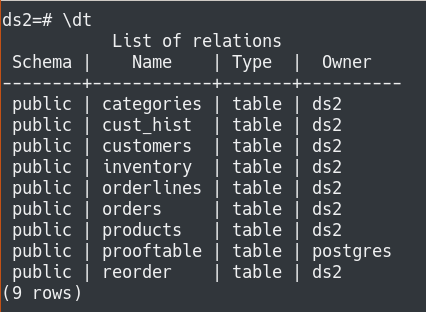
\includegraphics[width=0.8\linewidth]{images/table1}
	\figcaption{Tabellen können in pgAdmin eingesehen werden}
\end{minipage}	

Um nun das ERD (Entitiy Relational Diagram) zu sehen, wurde das Programm \verb|dbis| verwendet, um besagtes Diagramm zu erstellen:

\begin{minipage}{\linewidth}
	\centering
	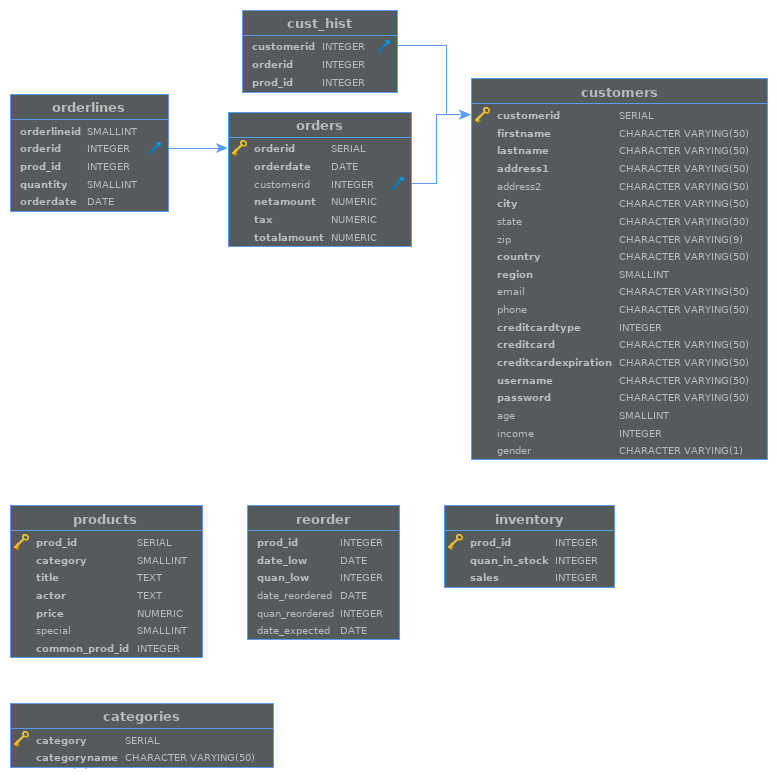
\includegraphics[width=1\linewidth]{images/tablevis}
	\figcaption{Tabellen wurden visualisiert und in Relation gestellt}
\end{minipage}

Durch dieses Diagramm kann analysiert werden wie die Fragmentierung gesetzt wird.
\subsection{Horizontale Fragmentierung}
Die horizontale Fragmentierung wurde so gesetzt, dass von den Bestellungen nur jene angezeigt werden, welche im ersten Halbjahr 2009 bestellt wurden und einen Nettobetrag über 300 haben. Der Sinn dahinter könnte sein, dass eine interne Analyse im Geschäft gemacht werden soll, bei welcher die analysiert wird wer im ersten Halbjahr große Einkäufe getätigt hat.

Der erste schritt ist ein horizontales Schema zu erstellen:

\begin{lstlisting}[language=SQL]
DROP SCHEMA IF EXISTS horizontal;

CREATE SCHEMA horizontal;
\end{lstlisting}

Danach wird in dem Schema ein Fragment als Tabelle erstellt. Eine Fragmentstabelle kann am angenehmsten mit folgender Syntax erstellt werden: \verb|CREATE TABLE schema.fragment AS (...)|, wobei nach \verb|AS| eine SELECT-Abfrage steht welche anschließend das Fragment darstellt. Für den vorhin beschriebenen Fall sieht es so aus:

\begin{lstlisting}[language=SQL]
CREATE TABLE horizontal.firstHalfYearBigger300 AS (SELECT * FROM orders WHERE netamount > 300 AND orderdate < '2009-07-01');
\end{lstlisting}

\begin{minipage}{\linewidth}
	\centering
	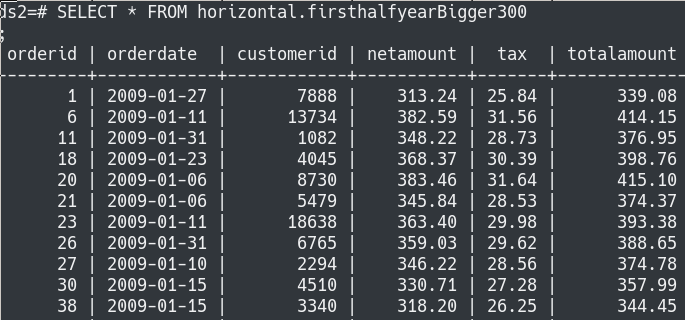
\includegraphics[width=0.8\linewidth]{images/table2}
	\figcaption{SELECT * FROM horizontal.firstHalfYearBigger300;}
\end{minipage}
\subsection{Vertikale Fragmentierung}
Für die vertikale Fragmentierung war die Idee Regalprodukte zu erstellen, welche lediglich Titel, Preis und natürlich die ID beinhalten. Nach dem Erstellen des Schemas namens \verb|vertical| wurde folgendes Fragment erstellt:

\begin{lstlisting}[language=SQL]
CREATE TABLE vertical.shelfProducts AS (SELECT prod\_id, title, price FROM products);
\end{lstlisting}

\begin{minipage}{\linewidth}
	\centering
	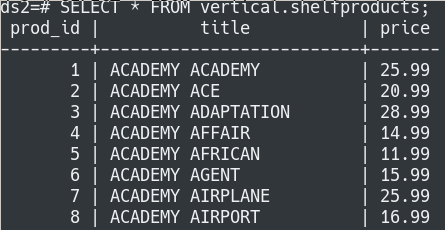
\includegraphics[width=0.5\linewidth]{images/table3}
	\figcaption{SELECT * FROM vertical.shelProducts;}
\end{minipage}
\subsection{Kombinierte Fragmentierung}
Für die kombinierte Fragmentierung wurde ein Konzept überlegt, bei welchem wieder von den Bestellungen horizontal geteilt wird indem dass erste Halbjahr genommen wird und Bestellungen welche einen Nettobetrag über 300 haben. Vertikal wurde nun nach dem Steuergeldbetrag und Gesamtbetrag, und natürlich ID gefiltert, um eine staatliche Analyse der großen Einkaufe zu bewerkstelligen.

Es wurde wieder ein Schema erstellt, namens \verb|combined|:

\begin{lstlisting}[language=SQL]
CREATE TABLE combined.firstHalfYearBigger300Tax AS (SELECT orderid, tax, totalamount FROM orders WHERE netamount > 300 AND orderdate < '2009-07-01');
\end{lstlisting}

\begin{minipage}{\linewidth}
	\centering
	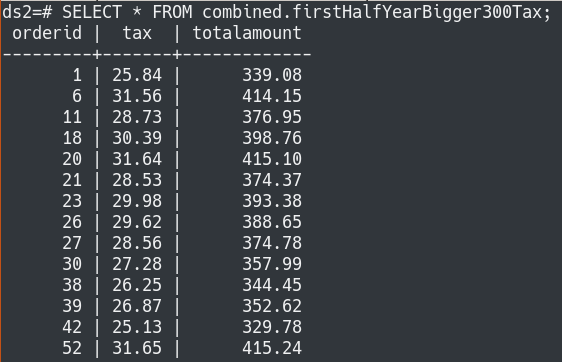
\includegraphics[width=0.8\linewidth]{images/table4}
	\figcaption{SELECT * FROM combined.firstHalfYearBigger300Tax;}
\end{minipage}
\subsection{Testung}
Um zu testen, mussten zuerst alle Gegenfragmente der jeweiligen Tabellen erstellt werden, um wieder die gesamte Tabelle zusammenfügen zu können
\subsubsection{Horizontal}
\begin{lstlisting}[language=SQL]
CREATE TABLE horizontal.secondHalfYearBigger300 AS (SELECT * FROM orders WHERE netamount > 300 AND orderdate >= '2009-07-01');

CREATE TABLE horizontal.firstHalfYearSmaller300 AS (SELECT * FROM orders WHERE netamount <= 300 AND orderdate < '2009-07-01');

CREATE TABLE horizontal.secondHalfYearSmaller300 AS (SELECT * FROM orders WHERE netamount <= 300 AND orderdate >= '2009-07-01');
\end{lstlisting}

Bei der horizontalen Fragmentierung müssen alle Fragmente mit \verb|UNION| zusammengefügt werden und anschließend werden diese gezählt und vergleicht mit der originalen Anzahl der orders:

\begin{lstlisting}[language=SQL]
SELECT COUNT(*) FROM (SELECT * FROM horizontal.firstHalfYearBigger300 UNION SELECT * FROM horizontal.secondHalfYearBigger300 UNION SELECT * FROM horizontal.firstHalfYearSmaller300 UNION SELECT * FROM horizontal.secondHalfYearSmaller300) AS "sub";

SELECT COUNT(*) FROM orders;
\end{lstlisting}
\subsubsection{Vertical}
\begin{lstlisting}[language=SQL]
CREATE TABLE vertical.otherProducts AS (SELECT prod_id, category, actor, special, common_prod_id  FROM products);
\end{lstlisting}

Bei der vertikalen kann geprüft werden, indem die Attribute der Tabelle verglichen werden. Zusammengefügt wird nicht mit \verb|UNION| sondern mit \verb|NATURAL JOIN|:

\begin{lstlisting}[language=SQL]
CREATE Table vertical.proofTable AS (SELECT * FROM vertical.shelfProducts NATURAL JOIN vertical.otherProducts);

-- Originale Tabelle
\d products
-- Beweis tabelle
\d proofTable

\end{lstlisting}
\subsubsection{Combined}
\begin{lstlisting}[language=SQL]
CREATE TABLE combined.firstHalfYearBigger300Tax AS (SELECT orderid, tax, totalamount FROM orders WHERE netamount > 300 AND orderdate < '2009-07-01');

CREATE TABLE combined.secondHalfYearBigger300Tax AS (SELECT orderid, tax, totalamount FROM orders WHERE netamount > 300 AND orderdate >= '2009-07-01');

CREATE TABLE combined.firstHalfYearSmaller300Tax AS (SELECT orderid, tax, totalamount FROM orders WHERE netamount <= 300 AND orderdate < '2009-07-01');

CREATE TABLE combined.secondHalfYearSmaller300Tax AS (SELECT orderid, tax, totalamount FROM orders WHERE netamount <= 300 AND orderdate >= '2009-07-01');

CREATE TABLE combined.otherOrders AS (SELECT orderid, orderdate, customerid, netamount FROM orders);
\end{lstlisting}
Bei combined müssen zuerst die Zeilen mit \verb|UNION| zusammengefügt werden, und anschließend mit \verb|NATURAL JOIN|:

\begin{lstlisting}[language=SQL]
CREATE Table combined.taxOrders AS (SELECT * FROM combined.firstHalfYearBigger300Tax UNION SELECT * FROM combined.secondHalfYearBigger300Tax UNION SELECT * FROM combined.firstHalfYearSmaller300Tax UNION SELECT * FROM combined.secondHalfYearSmaller300Tax);

DROP TABLE IF EXISTS combined.proofTable;
CREATE TABLE combined.proofTable AS (SELECT * FROM combined.taxOrders NATURAL JOIN combined.otherOrders);

-- Sollte das gleiche Ergebnis wie von SELECT COUNT(*) FROM orders; sein
SELECT COUNT(*) FROM combined.proofTable;
\end{lstlisting}

\section{Fragestellungen}
\subsection{Was versteht man unter dem Begriff Allokation beim Entwurf einer verteilten Datenbank?}
Es wird zwischen Fragmentierung und Allokation unterschieden. Anstatt wie bei Fragmentierung, enthalten bei Allokation die Daten verschiedenes Zugriffsverhalten indem diese verschiedenen Stationen zugeordnet werden.
\subsection{Beschreiben Sie die Korrektheitsanforderungen bei der Fragementierung von verteilten Datenbanken.}
\begin{itemize}
	\item \textbf{Rekonstruierbarkeit}: die Ursprungsrelation lässt sich aus den Fragmenten wiederherstellen
	\item \textbf{Vollständigkeit}: jedes Datum ist einem Fragment zugeordnet
	\item \textbf{Disjunktheit}: Fragmente überlappen sich nicht, d.h. ein Datum ist nicht mehreren Fragmenten zugeordnet
\end{itemize}
\subsection{Wie geht man bei einer horizontalen DB-Fragemtierung vor? Beantworten Sie diese Frage anhand eines Beispiels.}
\textit{Zerlegung einer Relation in disjunkte Tupelmengen, Zerlegung durch Selektionen}

Dabei ist gemeint, die Menge in Fragmente zu teilen, um diese auf verschiedene Standorte zu verteilen oder andere Gründe aufzuteilen. Beispiel könnte eine Tabelle sein, welche Preise enthält, könnte horizontal geteilt werden, wenn der Preis größer als 500 ist.
\subsection{Die Transparenz von verteilten Datenbanken ist in mehrere Stufen gegliedert. Beschreiben Sie die Lokale-Schema-Transparenz.}
\begin{itemize}
	\item \textbf{Fragmentierungstransparenz}
	\item \textbf{Allokationstransparenz}
	\item \textbf{Lokale Schema-Transparenz}: Benutzer muss Fragment als auch Standort kennen
\end{itemize}
\subsection{Was versteht man unter dem Begriff Fragmentierung beim Entwurf einer verteilten Datenbank? Wie sieht eine vertikale Fragmentierung aus? Erklären Sie die Begriffe anhand von einem Beispiel.}
Unter Fragmentierung versteht man das Aufteilen der Datenbank.

Das Problem bei der vertikalen Fragmentierung ist der Verstoß gegen die Rekonstruierbarkeit. Man lässt es zu, solange folgende Kriterien gelten:

\begin{itemize}
	\item Jedes Fragment enthält Primärschlüssel
	\item Jedem Tupel der Originalrelation wird künstlicher Surrogatschlüssel zugewiesen, der in Fragment übernommen wird
\end{itemize}

Ein Beispiel wäre, eine Tabelle mit sehr vielen Attributen zu haben, aus welcher man nur einige bestimmte Attribute in einer anderen Tabelle haben will. Beispielsweise könnte man aus Kontaktetabelle nur die E-Mails und Namen haben wollen, um an diese Briefe zu senden.